\chapter{Cooperative formations}

This chapter covers testing of different platooning cooperative actions – overtaking - and its effect on maximum capacity, average speed in real traffic conditions of Traffic model \#1, \#2 and number of dangerous situations of Traffic model \#1, \#2. 

For all tests in this chapter we switched off the decomposition of platoon in dangerous situation described in Section 4.2.4 for Snake overtaking type, to measure how dangerous are the non-cooperative and cooperative overtaking actions. The dangerousness is described by number of collision per hour and we evaluated it in all simulated environment, so in our case, for two or three-lane highway of length 5 km.

\section{Types of changing of lanes}

In the simulator there are programmed 3 types of overtaking and in Chapter 4 there is functionality description. In this section we did little conceptual overview of advantages and disadvantages, as well as some expected effects on a traffic.

\subsection{Snake}

Snake type of changing of lane is the easiest type of this action. It is non-cooperative action which depends only on decision of Lead vehicle of the platoon, so the lead vehicle do not any worry about the state of other following vehicles in the platoon.

Because all vehicles of platoon do the same action (changing of lane) at the same point of highway there is a risk, that the lead platoon vehicle driver does not properly estimate overtaking distance for whole platoon, it means that overtaking distance of each following vehicle in the platoon does not satisfy the safety rules. This type of overtaking action is safety for overtaking of a standing object, but not for overtaking of a moving object. The moving overtaken vehicle can get pretty close to the point, where the lead vehicles made back changing of lane from left to right lane and also each following platoon vehicle should make changing of lane. So it is necessary that each vehicle of the platoon has to evaluate possible collision all time during this operation. In order to minimize this danger there should be a such control module in each vehicle of platoon. And if it is not possible to make back changing of lane for some following platoon vehicle, then this vehicle must splits the platoon and becomes from the following vehicle into lead vehicle of newly created platoon to eliminate the collision situation.

There are still some other conceptual problems. Example of such problems is unexpected taking over the control of the following vehicle by its driver, because following platoon vehicle is managed “semi automatically by platoon”. The lead vehicle driver starts a “dangerous” overtaking or changing of lane and the following vehicle driver will respect safety rules and did not follow lead vehicle. 

If the decomposition of platoon is switched off in simulator, collisions will dramatically made the overtaken vehicle to decrease its speed. It would be reflected in simulator by decreasing of average speed.

\subsection{All at once}

It is cooperative changing of lane action which assumes reciprocal to each other knowledge of traffic situation of all platoon vehicles. As the name says the platoon can overtake only if no vehicle of platoon would not be endanger. All vehicles change the lane at same time. This changing of lane action should not finish by decomposition of platoon.

On the other hand, changing of lane All at once needs more free space for this action. Platoon of 6 vehicles with their length 4 meters and distances between vehicles 6m, need 50 meters and more of free space then overtaking action by single vehicle. It can result at deadlock between slow vehicles (trucks) in higher level of traffic density. It could decrease maximum capacity of highway and the average speed too.

\subsection{Last first}

This type of cooperative overtaking action is a hybrid between Snake type and All at once type and it consist of two steps. If lead vehicle decides about overtaking, the last following vehicle does changing of lane as first one if safety conditions are not broken. Then if it is possible all rest platoon vehicles change the lane too. If the first action, changing of line by last vehicle,  is safely done then the changing of lane by all platoon vehicles could  be done in  smaller free space. The last vehicle also “protect” rest platoon vehicles from some faster vehicles which are back in the lane. These “faster vehicles” should slow down for “short time”.

Unlike All at once overtaking, this Last first concept should increase capacity and average speed, because of easier changing of lane.






\newpage
\section[Experiment \#7: Maximum capacity of two-lane highway with real traffic and cooperative platooning]{Experiment \#7: Maximum capacity of two-lane highway with real traffic and cooperative platooning\sectionmark{Experiment \#7...}}
\sectionmark{Experiment \#7...}

According to Section 6.1 we expected little decrease of maximum capacity of highway.



\subsection*{Simulator setting for the test}
\begin{itemize}
\item Average speed: 34 m/s
\item Speed dispersion: 3 m/s
\item Length of platoon: 2-6
\item Number of lanes:  2
\item Platooning vehicles ratio: 0\%, 20\%, 40\%, 60\%, 80\%, 100\%
\item Generation limit: false
\item Generate trucks: true
\item Percentage of passenger vehicles in traffic: 67\%
\item Overtaking: Snake type, All at once type, Last fist type
\end{itemize}



\subsection*{Experiment results}

In Figure \ref{fig:6_2_2-1} there is dependency between maximum capacity of two-lane highway and percentage of platooning vehicles. This Experiment proved a negative effect of cooperative formation on maximum capacity of highway in higher level of percentage of platooning vehicles. 

For changing of lane by type All at once we supposed such result, because it is necessary to have more space for overtaking, but for Last first changing of lane we expected a little better results, but the values are smaller than type Snake.


In Figure \ref{fig:6_2_2-2} can be seen the difference of collision potential between cooperative and non-cooperative changing of lane.

\begin{figure}[!htbp]
\centering
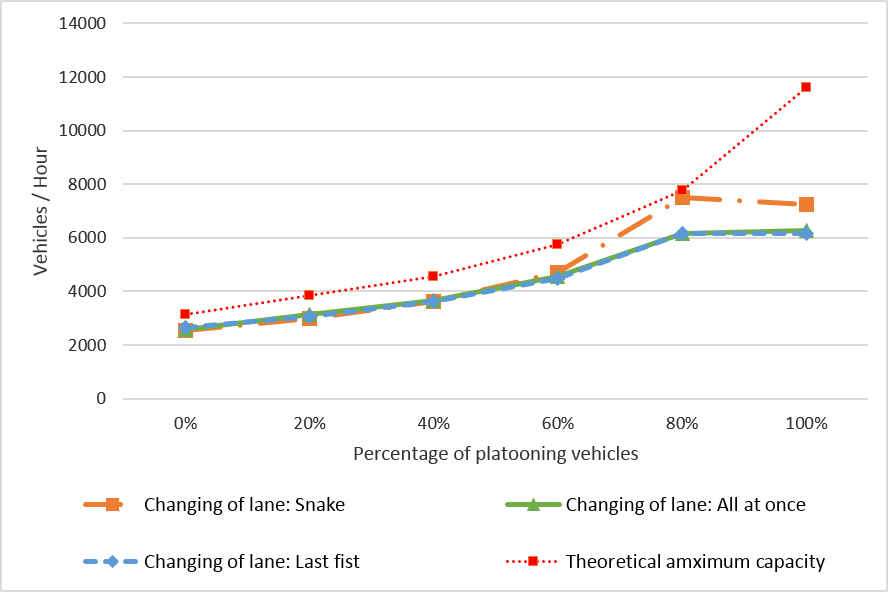
\includegraphics[width=0.82\textwidth,height=0.82\textheight,keepaspectratio]{figures/Chapter_6/6_E1_maxCap.png}
\centering
\protect\caption[Maximum capacity of two-lane highway with cooperate platoons]{\label{fig:6_2_2-1}Maximum capacity of two-lane highway with cooperative platoons - capacity measured only for 0\%, 20\%, 40\%, 60\%, 80\%, 100\% platooning vehicles, so as to be more visual the line connecting measured data was added.}
\end{figure}

\begin{figure}[!htbp]
\centering
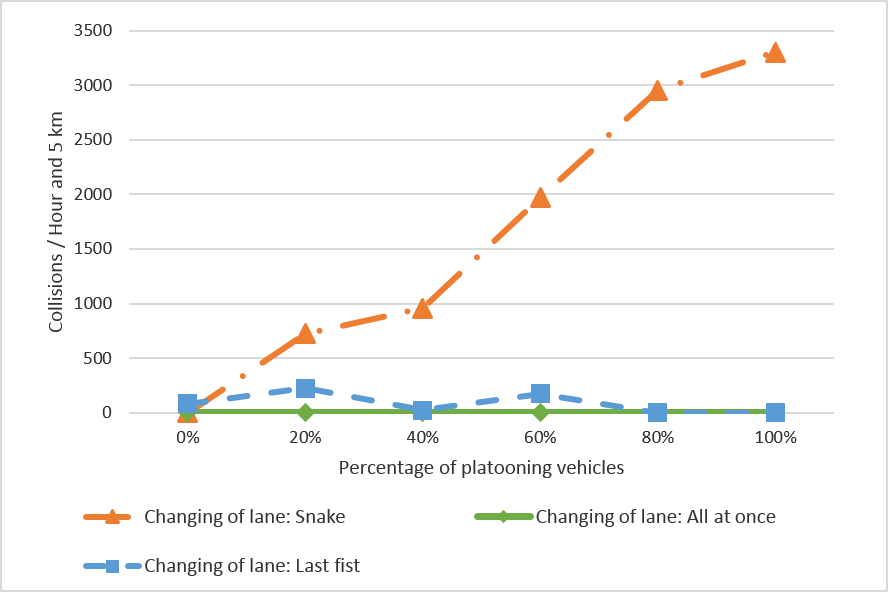
\includegraphics[width=0.82\textwidth,height=0.82\textheight,keepaspectratio]{figures/Chapter_6/6_E1_collision.png}
\centering
\protect\caption[Collisions per hour in simulated environment in simulated environment of maximum capacity of two-lane highway]{\label{fig:6_2_2-2}Collisions per hour in simulated environment in simulated environment of maximum capacity of two-lane highway - collisions measured only for 0\%, 20\%, 40\%, 60\%, 80\%, 100\% platooning vehicles, so as to be more visual the line connecting measured data was added.}
\end{figure}










\newpage
\section[Experiment \#8: Maximum capacity of three-lane highway with real traffic and cooperative platooning]{Experiment \#8: Maximum capacity of three-lane highway with real traffic and cooperative platooning\sectionmark{Experiment \#8...} }
\sectionmark{Experiment \#8...}

According to Section 6.1 we expected little decrease of maximum capacity of highway.


\subsection*{Simulator setting for the test}
\begin{itemize}
\item Average speed: 34 m/s
\item Speed dispersion: 3 m/s
\item Length of platoon: 2-6
\item Number of lanes:  3
\item Platooning vehicles ratio: 0\%, 20\%, 40\%, 60\%, 80\%, 100\%
\item Generation limit: false
\item Generate trucks: true
\item Percentage of passenger vehicles in traffic: 67\%
\item Overtaking: Snake type, All at once type, Last fist type
\end{itemize}



\subsection*{Experiment results}

In Figure \ref{fig:6_3_2-1} show us very similar results as in Experiment \#7, which proves the same negative effect of cooperative formation on maximum capacity of highway.




\begin{figure}[!htbp]
\centering
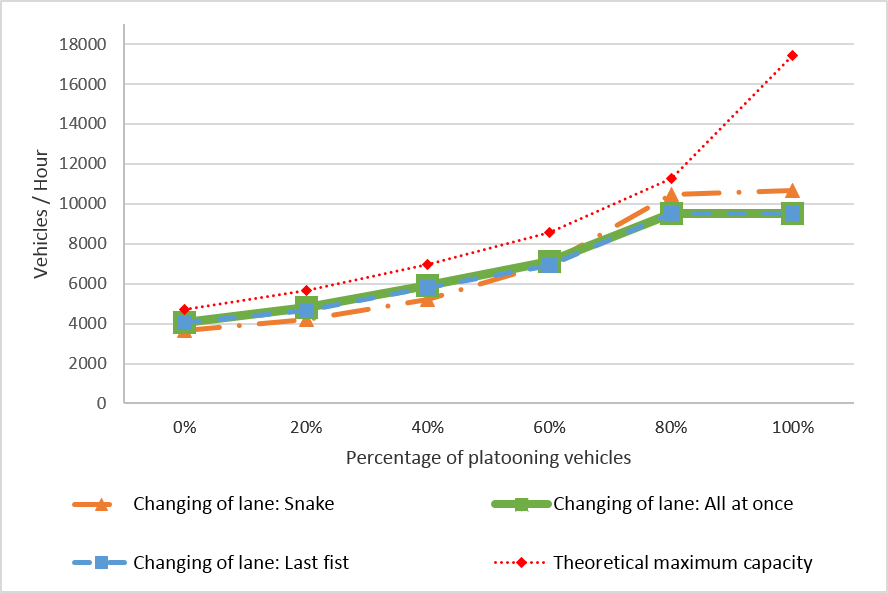
\includegraphics[width=0.82\textwidth,height=0.82\textheight,keepaspectratio]{figures/Chapter_6/6_E2_maxCap.png}
\centering
\protect\caption[Maximum capacity of three-lane highway with cooperate platoons]{\label{fig:6_3_2-1}Maximum capacity of three-lane highway with cooperate platoons - capacity measured only for 0\%, 20\%, 40\%, 60\%, 80\%, 100\% platooning vehicles, so as to be more visual the line connecting measured data was added.}
\end{figure}










\newpage
\section[Experiment \#9: Effect of cooperative platooning concept on traffic model \#1]{Experiment \#9: Effect of cooperative platooning concept on traffic model \#1\sectionmark{Experiment \#9...} }
\sectionmark{Experiment \#9...}

Overall positive effect of both cooperative and non-cooperative platooning was confirmed by previous experiments. We wanted also to test an effect of cooperative platooning on our real Traffic models.

\subsection*{Simulator setting for the test}
Settings of Traffic model \#1.
\begin{itemize}
\item Average speed: 34 m/s
\item Speed dispersion: 3 m/s
\item Length of platoon: 2-6
\item Number of lanes:  3
\item Platooning vehicles ratio: 0\%, 20\%, 40\%, 60\%, 80\%, 100\%
\item Generation limit: 3200 vehicles/hour
\item Generate trucks: true
\item Percentage of passenger vehicles in traffic: 67\%
\item Overtaking: Snake type, All at once type, Last fist type
\end{itemize}


\subsection*{Experiment results}

Based on our tests, with very similar results as in Figure \ref{fig:6_4_2-1} we were not able to confirm the assumption of increasing average speed of passenger vehicles by cooperative changing of lane in Traffic model \#1. But the cooperative approach had positive effect on safety of traffic in Traffic model \#1 (Figure \ref{fig:6_4_2-2}). The All at once changing of lane had zeros level of collisions but the unfortunately Last fist concept had some troubles. It was probably  due by a mistake in our simulator.


\begin{figure}[ph]
\centering
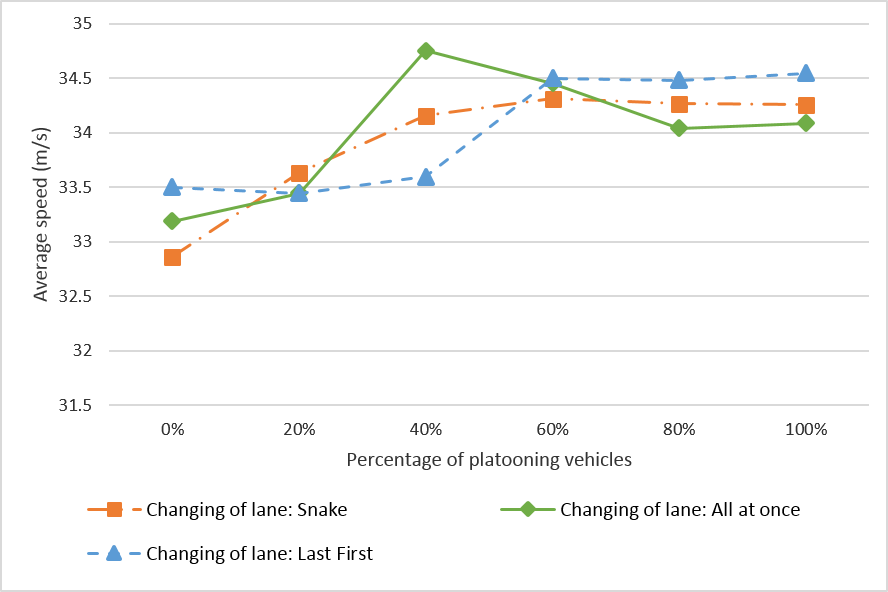
\includegraphics[width=0.82\textwidth,height=0.82\textheight,keepaspectratio]{figures/Chapter_6/6_E3_avgSpeed.png}
\centering
\protect\caption[Average speed of Traffic model \#1 with cooperative platoons]{\label{fig:6_4_2-1}Average speed of Traffic model \#1  with cooperative platoons - average speed measured after stabilization of traffic and only for 0\%, 20\%, 40\%, 60\%, 80\%, 100\% platooning vehicles, so as to be more visual the line connecting measured data was added.}
\end{figure}

\begin{figure}[!htbp]
\centering
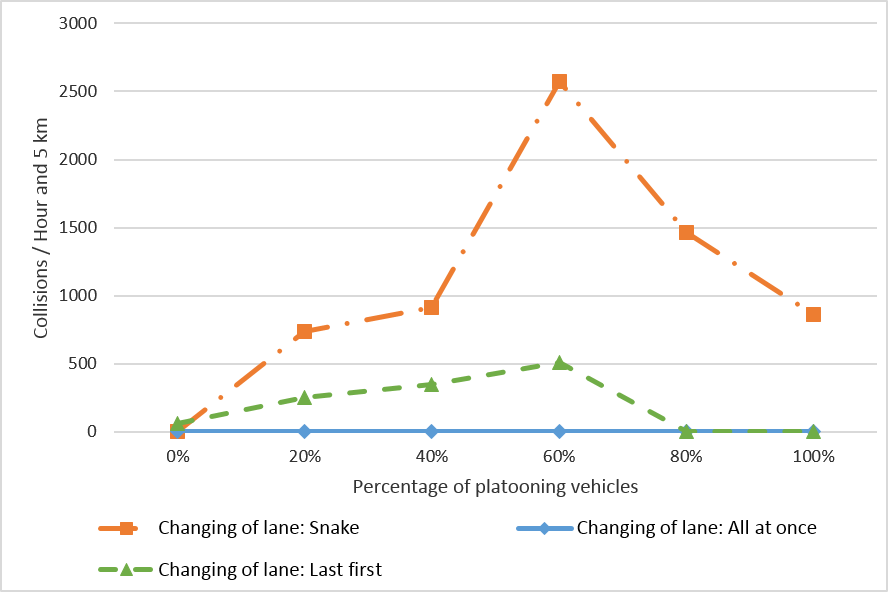
\includegraphics[width=0.82\textwidth,height=0.82\textheight,keepaspectratio]{figures/Chapter_6/6_E3_collision.png}
\centering
\protect\caption[Collisions per hour in simulated environment  of Traffic model \#1 with cooperative platoons]{\label{fig:6_4_2-2}Collisions per hour in simulated environment  of Traffic model \#1 with cooperative platoons - collisions measured only for 0\%, 20\%, 40\%, 60\%, 80\%, 100\% platooning vehicles, so as to be more visual the line connecting measured data was added.}
\end{figure}







\newpage
\section[Experiment \#10: Effect of cooperative platooning concept on traffic model \#2]{Experiment \#10: Effect of cooperative platooning concept on traffic model \#2\sectionmark{Experiment \#10...} }
\sectionmark{Experiment \#10...}

We also tested effect of cooperative changing of lane in Traffic model \#2.

\subsection*{Simulator setting for the test}
Settings of Traffic model \#2.
\begin{itemize}
\item Average speed: 34 m/s
\item Speed dispersion: 3 m/s
\item Length of platoon: 2-6
\item Number of lanes:  2
\item Platooning vehicles ratio: 0\%, 20\%, 40\%, 60\%, 80\%, 100\%
\item Generation limit: 1650 vehicles/hour
\item Generate trucks: true
\item Percentage of passenger vehicles in traffic: 67\%
\item Overtaking: Snake type, All at once type, Last fist type
\end{itemize}


\subsection*{Experiment results}

This experiment gave us some similar results as Experiment \#9 (Figure \ref{fig:6_5_2-1} and Figure \ref{fig:6_5_2-2}). We were not able to confirm expected increase of average speed, but again cooperation had positive effect on traffic safety.


\begin{figure}[ph]
\centering
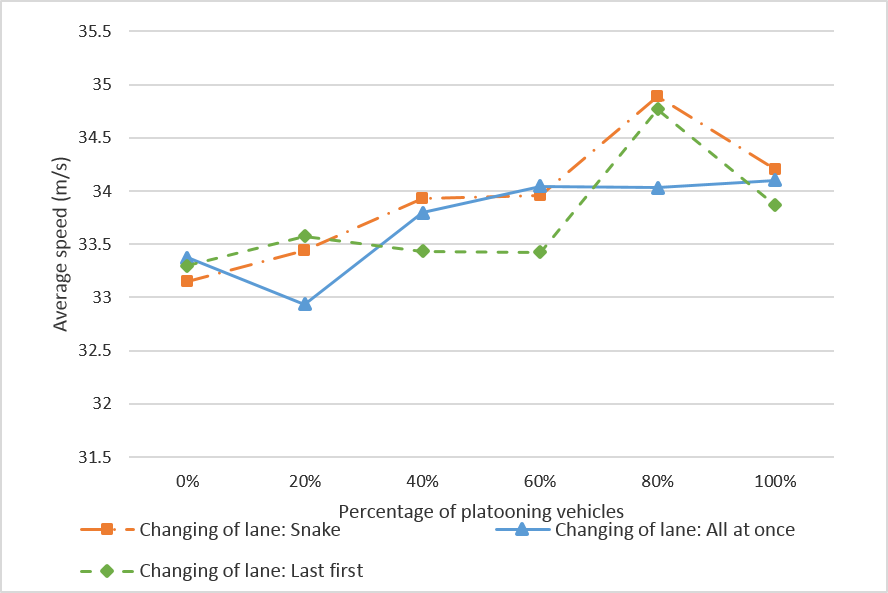
\includegraphics[width=0.82\textwidth,height=0.82\textheight,keepaspectratio]{figures/Chapter_6/6_E4_avgSpeed.png}
\centering
\protect\caption[Average speed of Traffic model \#2 with cooperative platoons]{\label{fig:6_5_2-1}Average speed of Traffic model \#2 with cooperative platoons - average speed measured after stabilization of traffic and only for 0\%, 20\%, 40\%, 60\%, 80\%, 100\% platooning vehicles, so as to be more visual the line connecting measured data was added.}
\end{figure}

\begin{figure}[ph]
\centering
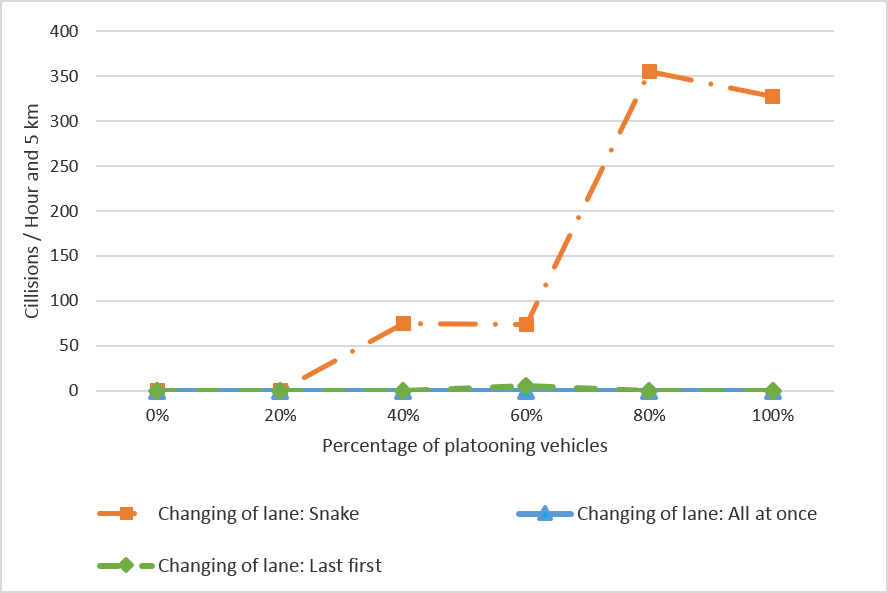
\includegraphics[width=0.82\textwidth,height=0.82\textheight,keepaspectratio]{figures/Chapter_6/6_E4_collision.png}
\centering
\protect\caption[Collisions per hour in simulated environment  of Traffic model \#2 with cooperative platoons]{\label{fig:6_5_2-2}Collisions per hour in simulated environment  of Traffic model \#2 with cooperative platoons - collisions measured only for 0\%, 20\%, 40\%, 60\%, 80\%, 100\% platooning vehicles, so as to be more visual the line connecting measured data was added.}
\end{figure}
